\documentclass[11pt]{article}
\usepackage[a4paper, hmargin={2.8cm, 2.8cm}, vmargin={2.5cm, 2.5cm}]{geometry}
\usepackage{eso-pic} % \AddToShipoutPicture
\usepackage{graphicx} % \includegraphics
\usepackage{listings}
\usepackage{setspace}
\usepackage{cite}

\lstset{
  moredelim=[is][\underbar]{_}{_}
}
%\usepackage{thebibliography}

\definecolor{Background}{rgb}{0.98,0.98,0.98}
\lstset{
    numbers=left,
    numberstyle=\footnotesize,
    numbersep=1em,
    xleftmargin=1em,
    framextopmargin=2em,
    framexbottommargin=2em,
    showspaces=false,
    showtabs=false,
    showstringspaces=false,
    frame=l,
    tabsize=4,
    % Basic
    basicstyle=\ttfamily\small\setstretch{1},
    backgroundcolor=\color{Background}
}

\author{
  \Large{Anna Sofie Kiehn and Henriks Urms}\\
  \\ \textit{Supervisor:} Martin Elsman
  % \texttt{a.kiehn89@gmail.com} \\
  %\\ \texttt{a.kiehn89@gmail.com} \\ \\
  %\Large{Henriks Urms}
  %\\ \texttt{urmshenrik@gmail.com}
}

\title{
  \vspace{5cm}
  \Huge{Midvejsrapport} \\
  \Large{Compiling TAIL to Futhark}
}

\begin{document}

%% Change `ku-farve` to `nat-farve` to use SCIENCE's old colors or
%% `natbio-farve` to use SCIENCE's new colors and logo.
\AddToShipoutPicture*{\put(0,0){\includegraphics*[viewport=0 0 700 600]{include/natbio-farve}}}
\AddToShipoutPicture*{\put(0,602){\includegraphics*[viewport=0 600 700 1600]{include/natbio-farve}}}

%% Change `ku-en` to `nat-en` to use the `Faculty of Science` header
\AddToShipoutPicture*{\put(0,0){\includegraphics*{include/nat-en}}}

\clearpage\maketitle
\thispagestyle{empty}

\newpage

\abstract

\newpage

\tableofcontents

\newpage

%%%%%%%%%%%%%%%%%%%%%%%%%%%%%%%%%%%%%%%%%%%%%
%%%%%%%%%%%%%%%%%%%%%%%%%%%%%%%%%%%%%%%%%%%%%
%%%%%%%%%%%  REPORT STARTS HERE  %%%%%%%%%%%%%%%%%%%%
%%%%%%%%%%%%%%%%%%%%%%%%%%%%%%%%%%%%%%%%%%%%%
%%%%%%%%%%%%%%%%%%%%%%%%%%%%%%%%%%%%%%%%%%%%%
\section{Prelude}

\subsection{Problem Definition}
Is it possible, effectively to compile TAIL programs, produced by the APL compiler AplTail,
into Futhark programs and thereby make use of the Futhark infrastructure for optimisation
and the possibility for targeting parallel hardware?

\subsection{Problem Elaboration}
The language APL is a mature array programming that gives rise to parallelism. The AplTail compiler produces
a typed intermediate language TAIL from APL source code. It also possible express parallelism in Futhark source code,
we wish to assess the possibility of compiling TAIL to Futhark thereby making it possible to execute APL in parallel through
the Futhark backend.

\section{Methods and tools}
In this section we will describe the methods and tools used to create the compilitalion scheme and implementation of the  compiler. 

\subsection{Symbolic notation describe the compilation scheme}
We are going to use a symbolic notation to illustrate a compilation scheme showing the compilation in a way that abstracts away implementation details. We use this tool to create a description of the compilation scheme that is independent of the implementation and which should make it possible to implement the compiler in any language.

\subsection{Parser}
We used a parser that was created douring an earlier project \cite{APLACC} instead of creating our own. This was done in order to use alredy existing tools and save our resources for work that had not alredy been done by others. We did however have to update the parser a little as it was a few months old and therefore did not support the newest additions to the TAIL language. Details about this implementation can be found in the section \textit{Implementation of the compiler}. 
We used an alredy existing compiler in order not to use our resources on work that had alredy been done, that way opening up more time to work on the actural compilation.

\subsection{Libaries used}
cabal, golden ...

\section{Project status}
The project is comming along as planed and we are keeping to our time schedule that can be seen in Figure \ref{fig:gantt}.
It took shorter time than expected to adabt the parser to work with the latest version of TAIL
which meant that we started on the implementation of the TAIL functions in the compiler a few days before sceduled. 
We are done with implementing half of the functions in TAIL to Futhark source code.As we are work on testing the
implementation while we develop we are halfway through testing the functionality as well. 

\begin{figure}[width=\textwidth]%[p]
    \centering
    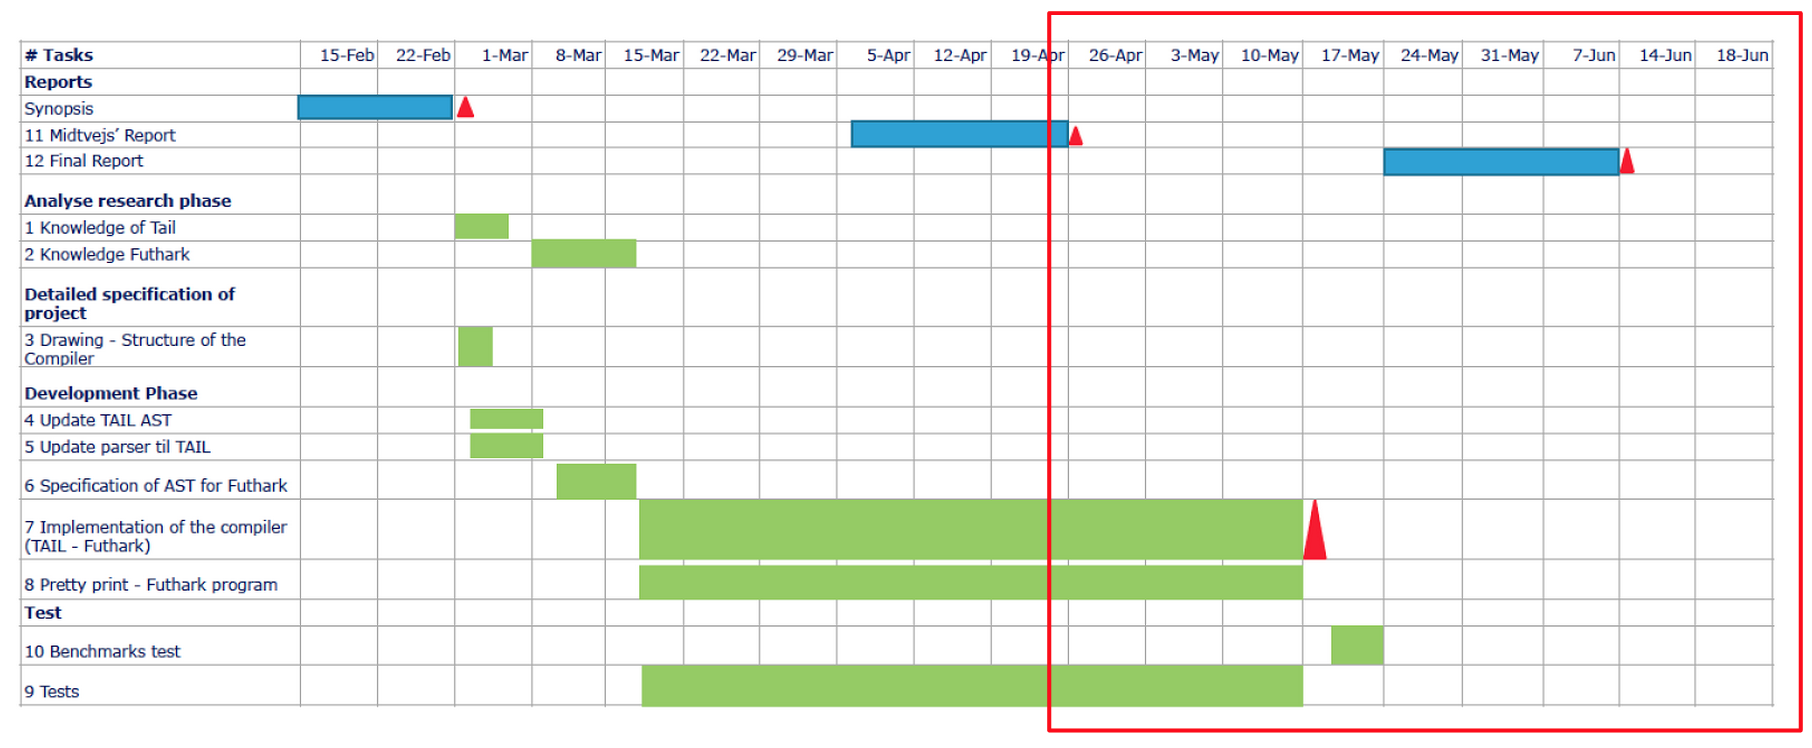
\includegraphics[width=\textwidth]{midvejsgantt3.png}
    \caption{Gantt chart of the project activities. The remaining time of the project is highlighted by a red box.}
    \label{fig:gantt}
\end{figure}

The compilation scheme we are going to create are still being developed. The symbolic notation is something we will work intensively on from now on. So far only a small portion have been written down in a symbolic notation, the rest is still described in a more informal text form. 
Besides this we will use the remaing time in the project we will focus on getting the last functions implemented and tested.

We will also test the efficiency of our generated Futhark code using benchmarks to compare it to the C-code generated by the TAIL compiler. 


\newpage

\section{Introduction}

In recent years, there has been a lot of focus on leveraging the power of parallel hardware. 
One approach has been to design programming languages with explicit data-parallel constructs that can be compiled 
into highly parallel code. One such language is Futhark. The aim of Futhark is to target parallel hardware such as 
GPUs while itself being the target of more programmer-productivity oriented languages. The Futhark compiler 
performs several optimizations, such as fusion, which enhance the degree of 
parallelism \cite{T.Henriksen&C.Oancea}.\\

APL is an array lanuage and includes various operations that are central to the language and are good candidates 
for parallel execution. Efforts in compiling APL to parallel backends already exist in the form of the language 
TAIL (Typed array intermediate language) and it’s compiler. The TAIL compiler captures the parallelism inherent in 
APL source code and brings it to a much more manageable form. In our work we provide a compiler from TAIL 
to Futhark thus bridging the gap between APL and Futhark.\\

The language Futhark is designed to target parallel architectures and at the same time acting 
as an intermediate language for more feature-rich languages. By compiling APL to Futhark through TAIL the 
Futhark compiler can be used to generate parallel code from APL once a parallel backend for 
Futhark is completed.\\

There are traditionaly five stages of a compiler if you compile a high level language to mashine code: 
lexical analysis, syntax analysis, type checking, intermididate code generation, register allocation, mashine 
code generation and assembly and linking \cite{TorbenMogensen}. However, in this project we are compiling from 
one high level language to another high level language. The structure does therefore look a little different. 
The first two phases are still lexical analysis and syntax analysisare and are handled by a parser. We made use of an alredy existing parser \cite{APLACC} and only modified it in order for it to work on the latest 
version of TAIL. The third phase is transforming the abstract syntax tree of TAIL to the abstract syntax tree 
representing the code in Futhark and the fourth phase is printing the AST so it becomes correct 
Futhark source code. \\

One of the main point of interest in the compilation between TAIL and Futhark is compiling the four array operators 
of TAIL: {\tt each}, {\tt eachV}, 
 {\tt reduce} and {\tt zipWith} to Futhark source code that include the four second-order array compinators in Futhark:  
 {\tt map}, {\tt filter}, {\tt reduce} and {\tt scan}. However as the functionality of these fuctions are not completly 
 identical the work lies in creating a mapping that retains the parallalism in the original code in the target language.\\
 This can be seen in the exaple below which illustrate this difference. The reduce function in the
  TAIL language is maped to a nested reduce function in the Futhark language.
  As some function names exists in both languages the futhark version of such uccurences are \underline{underlined}.

\begin{lstlisting}[numbers=none,frame=none]
reduce(+, [[1,2,3,4],[5,6,7,8]]))

  =>

_reduce_(fn x => map(+,x),[[1,2,3,4],[5,6,7,8,]])

\end{lstlisting}

This paper contributes with a compilation scheme that are implementation independent, showing a replicateble 
way of how to translate the typed intermididate language of APL, TAIL, to the functional language Futhark. Also 
this paper presents an implementation of the privius mentioned scheme in Haskell. The efficiency of this
 implementation have been tested by comparing benchmarks test on code generated by the C-backend to TAIL 
 and the generated Futhark source code by using the C-backend to Futhark. \\

The project is open source and the source code can be found here:\\ https://github.com/henrikurms/tail2futhark.

\section{TAIL}

TAIL is a typed array intermidiate language and the target of an APL compiler. APL is an older laguage created in the 1960's by Kenneth E. Iverson. APL is an array programming language, its main type is the multi-dimentional array 
and most of the bild in functions in the language are array operators that work on this type. 
All of its build-in functions or operators are represented by special graphic symbols allowing for very concise code.
The APL language is dynamicly typed. It support first and second order functions and it supports polymophism in 
both its first and second order functions and operators. 
Even though it is not a new language it is still used in the financial world 
where large code bases are still operational and activly developed \cite{MartinElsman}. \\

%Traditionaly APL is interpret .. \\
TAIL was designed with the purpose of targeting parallel architectures, though no parallel backend for TAIL yet exists. TAIL can also be compiled efficiently into a C-like language \cite{ElsmanDybdal:Array:2014}\\

The expressivity of TAILs type system allows the compiler to express some operators wich are primitive in APL such as the inner product operator using simpler operators. \\

The central type in taiil is the multi-dimentional array type. Array types consist of a base type and a rank. The base type of an array is the type of the elements in the array.  The currently supported base types are {\tt int}, {\tt double}, {\tt bool} {\tt char}. Scalars are arrays of rank 0. Most operators i TAIL are polymorphic in respect to array ranks and base types. 

Certain operators (such as shape) produce one dimensional array for wich the length is known at compile time. The types of such values are captured in a special vector type that keep track of the vector sizes. 
TAIL include special operators that operate on vectors and peserve this type information. 

The explicit types of TAIL is used to compile away some operators of APL, instead substituting them with simpler APL functions. \\

TAIL programs always consist of a single expression. SEE ARTICLE FOR REFERENCE \\

Below we discuss some selected operators from TAIL.

{\tt each} takes as arguments a kernel and an array and functions as the generel map, applying the kernel to each element in the flattened array. 
{\tt eachV} is a special case of {\tt each} ...\\
{\tt reduce} takes as arguments a kernel, a neural element and and array. It works similar to fold in ML starting by aplying the kernel to the neural element and the first element of the array and then the continuesly the kernel applied to the result and the next element in the array. 
{\tt zipWith} takes a kernel and two arrays. It then applies the kernel on the censecutive pair of elements consisting of the i-th element from the first array and the i-th element from the second array. 

%The types in TAIL are devided into four types. Firstly there are base types comsisting of {\tt int}, {\tt double}, {\tt bool} and the polymorphic type {\tt $\alpha$} that can represent any one of them. Secondly, there are shape types that can be either a scalar value/variable of type int,  or a shape variable or a combination of two shape variables. \\
%Then there is array types that consist of a base type and a rank. Finaly there is 


%The main datatype in TAIL is also a multidimantional array. Array types are in TAIL annotated with their ranks explicetly. 
%TAILs type system treats scalar values as special cases of the array time namly an array with rank 0. 

%There are two seperate representations of vectors, either the special vector type used when the length of the vector is known or the general array type where the rank is 1.  
 
%Besides array and vector types, TAIL also have base types in the form of {\tt int}, {\tt double}, {\tt bool} and {\tt $\alpha$}.

%So far TAIL only support a subset of the APL functions and operators. 

\section{Futhark}

Futhark is a functional programming language inspired by Haskell and Standard ML.
It was designed to be an attractive choice for expressing complex programs by having enough expressive power without
losing the posibility to do agressive optimization and creating parallelisation even though the higher the expressive power of the
language the more difficult optimization ofthen become.
Due to this the Futhark language only supports regular arrays (arrays where all inner dimentions are of the same length)
because of the complication to size analysis supporting non-regular arrays would create.
However Futhark do support nested parallalism as this is a feature many programs depend upon \cite{TroelsHenriksen}.\\

Futhark is a mostly first order language but supports bulk (parallel) operations on arrays
using the build-in second-order array combinators (SOACs) of the language. 
The SOACs consist of {\tt map}, {\tt filter}, {\tt reduce} and {\tt scan}.
The operators have the expected functionality also found in Haskell and Standard ML.
Futhark supports nesting of array types, an int array array will contain int arrays and so on.
{\tt map} maps a function onto each element in the array.
If the array mapped over contains arrays the function will be applied to each array,
so in other words the function is mapped over the outer-most dimension of the multi-dimensional array.
The language is expressive enough that the same functionality as these functions present can be created using do-loops
but that should be avoided do to the fact that the optimization Futhark make available are based on the
transformation on the four SOACs. \\

The basic types in Futhark is {\tt int}, {\tt char}, {\tt bool}, {\tt real} and regular arrays.
The type system of Futhark does not support polymorphism,
owever the build-in SOACs work on all regular arrays created of the basic types. 

%Does not support polymorfism in types

A Futhark program consist of a list of function declarations like
\begin{lstlisting}[numbers=none,frame=none]
fun return-type name(params...) = body
\end{lstlisting}

Except for inline anonymus functions all functions are defined globaly. 

\section{The differences between TAIL and Futhark}
The difficulty in compiling TAIL to Futhark is creating the same functionality in 

\subsection{Polymorphism}

\section{Compilation strategy}
As mentiont previusly a Tail program always consist of one single expression, whereas a Futhark program is a list of function declarations. The Tail expression is therefore translated/compiled to a Futhark expression by making it the body of the Futhark function. 
Thus the chalenge boils down to translating Tail expressions to Futhark expressions. 
There are 10 different kind of Tail expressions most of whitch has exact equivalents in the Futhark language. This includes but are not limited to, veriables, let ecpressions and litterals. Thus the interesting case is really if the expression is an operator expression. \\

These operators consist of the scalar operators: add, addi, subi, subd, multi, multd, mini, mind, maxi, maxd, andb, orb, xorb, nandb, norb, notb, lti, ltd, ltei, lted, gti, gtd, gtei, gted, eqi, eqd, negi, negd, i2d and b2i, and the array operators: iotaV, iota, eachV, each, reduce(V), reduce, shapeV, shape, reshape, reshape0, reverse, vreverse, rotateV, vrotateV, rotate, transp, transp2, takeV, take, dropV, drop, consV, cons, snocV, snoc, firstV, first, zipWith, catV and cat. \\

The scalar operators have equivalents in the Futhark language and are therefore straight forward to compile. Some of the Tail array operators also have eqivalent or almost eqivalent counterparts in the Futhark laguage but most have not and are therefore interesting to take a closer look at.

\section{The parallel operators}

\subsection{each}

The type of the {\tt each} function is $each(f,a) :: \forall\alpha\beta\gamma.(\alpha \to \beta) \to [\alpha]^\gamma \to [\beta]^\gamma$.

The {\tt each} function in TAIL applies a function to every element in the flat representation of the array. This is a completely parallel operation more commonly known as map. The {\tt map} combinator in futhark has slightly different semantics.
Since futhark views a multidimensional array as nested simple arrays it applies the function to every array element.
Thas is, it maps the function into the outer-most dimention of the array.

To solve this problem we have nested {\tt map}s to the depth of the array with the required function, for example, an {\tt each} operation over an array of rank 2 would have two {\tt map}s nested in each other so the kernel is mapped on each element of basic type.

For example an each operation on an array of rank 2 will look like:
\begin{lstlisting}[numbers=none,frame=none]
each(f,a)	=>	map(fn x => map (f,x), a)
\end{lstlisting}

This means the parallel {\tt each} operations in TAIL are compiled to parallel code in the futhark language.

\subsection{eachV}
The {\tt eachV } is just a special case of the {\tt each} operator that works on vectors, i.e. flat arrays where the size
is known at compile time. We do not use this extra information so this special case is not important for us.

\subsection{reduce}
The type of the {\tt each} function is $reduce(f,id,a) :: \forall\alpha\gamma.(\alpha \to \alpha \to \alpha) \to \alpha \to [\alpha]^{\gamma+1} \to [\alpha]^\gamma$.
The {\tt reduce} function in TAIL uses an associative binary operator to reduce an array of rank $\gamma+1$ to an array of rank $\gamma$ by reducing along the inner-most dimension. The futhark reduce on the other hand reduces each array in the outer array, i.e. it reduces along the outer-most dimension. 

We have adopted the samme approach as with each by using nested maps to map the reduce on the innermost dimension.

Fore example reducing an array of rank 2 emits the following code:

\begin{lstlisting}[numbers=none,frame=none]
reduce(+,a)	=> 	map(fn x => reduce(+,x), a)
\end{lstlisting}

\subsection{zipWith}

The zipWith operator applies a scalar binary operator on pairs of elements from two arrays of the same shape two
produce a third array of the same shape as the input arrays.

 To do this in futhark we use the zip function to convert two arrays to an array of tuples and map the binary operator on that array of tuples.

\section{Other interesting operators}

Beside the parallel operators there are other operators worth mentioning mostly because of non trivial semantics.  

\subsection{reshape}

The reshape operator also has quite unique semantics in TAIL, if the dimensions of reshape don't match the dimensions of the array, the
array is either truncated or the elements are repeated until the array is long enough.

Futhark has a reshape function that only works for arrays of the correct dimensions.

Our general strategy for compiling reshape is to first ensure that the array is the correct size and then use the futhark reshape
function to do the final step. To adjust the size we operate on the flat representation of the array, this is easy to produce also
using futhark reshape. To adjust the array we first make sure it is long enough by extending it using the function replicate and then
truncate it to the correct length with split.

To keep the implementation simple we generate code that calls generated library functions written in futhark which do most of the work.
Nevertheless we inline the flattening and reshaping code so we only need reshape functions written in futhark
for the one dimensional cases. If we wanted to simply call a function instead we would need a seperate library function for each
rank and basic type combination which we needed to call reshape on since futhark only allows declaration of monomorphic functions.

We have to decide where to put the library functions.
We would like the compiler to always output a valid (runnable) futhark program given a valid TAIL input program, so we would like to
be able to include the library in the output when we run the compiler.
Furthermore since futhark has no polymorphism we have to include versions of all types, but we would like to only maintain one version.
Finally since Funthark is eventually expected to feature polymorphism and a module system we would like the solution to not be too
extensive. Therefore we have coded the functions in the compiler itself.

We have used this approach throughout our compiler, e.g. the take operator is implemented similarily.

\subsection{take} 

The {\tt take} operator in TAIL has very unique semantics, for a positive arguement that is less than the size of the array it behaves as one would suspect i.e. it returns the first n elements of the array. For a negative argument {\tt take} returns the last n elements of the array. If there are not enough elements in the array, {\tt take} pads with zeros.

In a similar fashion to reshape we have used library functions do most of the work.
We flatten the array, let the library function work on the flat representation and finally reshape it to the desired shape.
This approach has all the benifits mentioned earlier.

\section{Implementation of the compiler}

\subsection{Adabtion of the parser}
The parser that we make use of was created in a precius project \cite{APLACC}. In the time between that project finished and ours commenced the TAIL language had been updated with new features and we therefore had to update the parser so that it worked with the latest version of TAIL.\\

One of the things that had changed was that boleans was added to the TAIL language. That meant that it had to be added ..\\

Another thing that had changed was that the shape type in the older version of TAIL was replaced with a vector type in the newer version.\\

\subsection{Description of the system}
Flags, test..
we expect that the tems we get in are well typed and correct. 

\section{Testing}
We have used two methods to test the compiler we have created. One is unit or integration test where we test the entire pipeline from giving it APL source code to running Futhark source code. The code is parsed whrough the APL to TAIL compiler \cite{ElsmanDybdal:Array:2014} through our compiler (TAIL to Futhark) and then through the Futhark compiler \cite{TroelsHenriksen} that returns a result, a result that is then compair to a file containing the expected result using the golden REFERENCE!!!!!!!! %\cite{}
libary. This form of testing will test the correctness of our code. \\

The second way are going to do testing is by benchmark test. This we will do in order to evaluate the efficiency of our code. 

\section{Discussion}

\subsection{No parallalism yet}

\subsection{The problem of polymorphism vs. no polymorphism}

\section{Summary and future work}



%%%%%%%%%%% REFERENCES  %%%%%%%%%%%%%%

\bibliography{references}{}
\bibliographystyle{plain}

There will be more references in the final thesis. 
\end{document}
